%%%%%%%%%%%%%%%%%%%%%%%%%%%%%%%%%%%%%%%%%%%%%%%%%%%%%%
% % Modelo de Monografia
% % Autor: Felipe Brunelli de Andrade - Mar�o 2010
%%%%%%%%%%%%%%%%%%%%%%%%%%%%%%%%%%%%%%%%%%%%%%%%%%%%%%

% % Defini��o da estrutura do documento, utilizando o ABNTex
% % Formato de impress�o frente-verso com come�o de cap�tulo em 
% % p�gina impar, com cabe�alho em cada p�gina com nome do cap�tulo
% % e n�mero de p�gina, A4 e fonte tamanho 12
\documentclass[espaco=duplo,brazil,ruledheader,a4paper,12pt,twoside]{article}
% % Pacotes para reconhecimento de acentos e hifeniza��o pt-br
\usepackage[brazil]{babel}
\usepackage[latin1]{inputenc}
% % \usepackage[dvips]{graphicx}
% % Pacote gr�fico para PDF
\usepackage[pdftex]{graphicx,lscape}
% % Estilo de refer�ncia para Bibliografia - Alfab�tico
%\usepackage{natbib}
\usepackage[pdftex,pdfpagelabels,plainpages=false,pagebackref,hyperfootnotes=false]{hyperref}
\hypersetup{colorlinks=true,linkcolor=blue,citecolor=blue,urlcolor=blue}
\usepackage[abnt-url-package=hyperref]{abnt-alf}
% % Pacote que prov� 11 simbolos matem�ticos
\usepackage{latexsym}
% % Pacote que permite a inclus�o de arquivos eps
\usepackage{psfrag}
% % pacote para adicionar endere�os eletr�nicos
\usepackage{url}
% % Pacote usado para listar Siglas e Simbolos
% \usepackage[estilo=UFPR]{tabela-simbolos}
\usepackage{tabela-simbolos}
% % Pacote semelhante ao minipage para inclus�o de figuras lado a lado
\usepackage{subfigure}
% % Pacote que auxilia em referencias - pouco usado
% \usepackage{varioref}
% % Suaviza��o de fonte
\usepackage{dsfont}
% % Pacote para adicionar espa�os quando necess�rio
% \usepackage{xspace}
% % Pacote que auxilia na cria��o de tabelas
% \usepackage{tabularx}
\usepackage{longtable}
\usepackage{multirow}
% % Pacote que ajuda a rotacionar elementos na p�gina
\usepackage{rotating}
% % Pacotes matem�ticos
\usepackage{amsmath}
\usepackage{amsfonts}
\usepackage{amssymb}
\usepackage{mathtools}

% % Macros - use se precisar
% \newcommand{\simb}[2][]{
% \ifthenelse{\equal{#1}{}}
% {\addcontentsline{los}{simbolo}{\ensuremath{#2}}}
% {\addcontentsline{los}{simbolo}{#1}}
% \ensuremath{#2}}
% \makeatletter
% \newcommand{\listadesimbolos}{
% \pretextualchapter{Lista de S�mbolos}
% {\setlength{\parindent}{0cm}
% \@starttoc{los}}}
% \newcommand\l@simbolo[2]{\par #1, p.\thinspace#2}
% \makeatother
% 
% \newcommand{\R}{\mathds{R}}
% \newcommand{\Cinf}{\mathcal{C}^\infty}
% \newcommand{\Cinfc}{\Cinf_c}

\begin{document}

% % Tipos de imagens para serem inseridas no texto
\DeclareGraphicsExtensions{.jpg, .pdf, .mps, .png, .tiff} 

% % Defini��o de vari�veis para utiliza��o no ABNTex
\renewcommand{\autor}[0]{Bruno Kim Medeiros Cesar, Daniel Luiz de Albuquerque}
\renewcommand{\titulo}[0]{Dissemina��o de informa��o em Redes Complexas}
\renewcommand{\local}[0]{S�o Carlos -- SP}
\renewcommand{\instituicao}[0]{UNIVERSIDADE DE S�O PAULO}
\newcommand{\instituto}[0]{Instituto de Ci�ncias Matem�ticas e de Computa��o}
\renewcommand{\data}[0]{Junho de 2013}

\begin{titlepage}

\newcommand{\lyxline}[1]{
  {#1 \vspace{1ex} \hrule width \columnwidth \vspace{1ex}}
}

% Documentos a serem incluidos na Monografia
\thispagestyle{empty}

% capa - come�o
\begin{center}
\Huge{\textsf{\instituicao}}\\
%\small{\textsf{\instituto}}
\end{center}

\vspace{6cm}

\lyxline{}
\begin{center}
\noindent
\Large{
\textsf{\titulo}}\\
\vspace{1em}
\noindent
{\bf \autor}
\end{center}
\lyxline{}

\vspace{7cm}

\begin{center}
\textsf{\local}
\end{center}

\cleardoublepage
% folha de rosto - comeco
%\begin{center}
%Copyright 2010 \autor.\\ %Este documento � distribu�do nos termos da licen�a descrita no arquivo LICENCA que o acompanha.
%\end{center}
%\newpage

\vspace*{1cm}

\begin{center}
\noindent
\Large{
\textsf{\titulo}}
\end{center}

\vspace{2cm}

\begin{center}
\noindent
\large{\bf {\it \autor}}\\
\vspace{1em}
\end{center}

\vspace{3cm}

\hfill{
\begin{minipage}{0.6\columnwidth}
{Monografia referente ao segundo trabalho para a mat�ria Redes Complexas para a Computa��o.}\\\\\\\\\\

\end{minipage}}

\vspace{1.5cm}

\begin{center}
\textsf{USP - S�o Carlos}\\
\textsf{\data} \\
%\textsf{(Vers�o Final Revisada)}
\end{center}

%\newpage\ 
% folha de rosto - fim

\cleardoublepage
\chapter*{Resumo}

\noindent{}Resumo aqui.


\end{titlepage}
% \tableofcontents
\sumario
\listoffigures
\listoftables

\begin{center}
\chapter*{Lista de Abreviaturas}
\end{center}

\singlespacing

\noindent
 
\begin{tabular}{p{2.5cm} p{12cm}}
RC & \textit{Redes Complexas}\\
\end{tabular}


\clearpage

\cleardoublepage

%\doublespacing

\pagenumbering{arabic}

\chapter{Introdu��o}

Processos de dissemina��o de informa��o s�o encontrados em muitas �reas do conhecimento, como na dispers�o de rumores,
propaga��o de v�rus digitais e biol�gicos, atualiza��o de estado em sistemas distribu�dos, e mesmo em processos 
f�sicos de dispers�o. O elemento comum entre todos estes fen�menos � a ocorr�ncia de uma atividade descentralizada,
onde cada agente interage com seus pares para alterar o estado global do sistema. A dissemina��o ent�o emerge
como um comportamento complexo com origem na intera��o entre agentes simples.

No primeiro trabalho da disciplina, examinamos diferentes modelos de dissemina��o de informa��o, 
provenientes das �reas de epidemiologia e sociologia. Tais modelos consistem na identifica��o de compartimentos
que correspondem a diferentes est�gios de uma epidemia, e o estabelecimento de regras para transi��o entre 
compartimentos, dependente ou n�o da intera��o entre indiv�duos. 

Tal abordagem prov� uma equa��o diferencial que pode ser solucionada por m�todos de integra��o num�rica, correspondendo
ao modelo idealizado de uma popula��o muito grande onde os indiv�duos se encontram aleatoriamente ao acaso. Tal abordagem
cont�nua permite um estudo anal�tico profundo das condi��es e resultados da dissemina��o, mas se baseia em um modelo de
intera��o - mistura completa - que n�o tem sentido em muitos processos reais.

O modelo de mistura completa assume que os indiv�duos possuem igual capacidade para interagir com quaisquer outros 
indiv�duos. � poss�vel implementar estratifica��es \textit{ad-hoc} adicionando mais compartimentos ao sistema, mas uma
abordagem mais promissora � simplesmente implementar o processo sobre uma rede que mapeia todas as rela��es poss�veis.
Deste modo, o modelo de mistura completa torna-se um caso especial, onde a rede � um grafo completo. Deste modo,
abandonam-se an�lises cont�nuas em favor da simula��o discreta, onde a rede oferece a topologia das intera��es.

Contudo, com isso adiciona-se uma nova camada de complexidade � an�lise, pois os efeitos da dissemina��o tamb�m dependem da 
estrutura da rede sobre a qual ela � executada. A pesquisa sobre esse tipo de processo din�mico ainda � 

Linkar trabalho anterior, Impacto dos modelos ded rede na propaga��o; M�tricas estruturais da rede como medida comparativa.  trabalho analisa propaga��o em diferentes aspectos: modelos de redes e redes reais;

\chapter{Revis�o Bibliogr�fica}

O estudo de Redes Complexas � a base para a compreens�o da complexidade, buscando explicar a emerg�ncia e 
evolu��o estrutural do esqueleto de um sistema complexo \cite{barabasi2007architecture}. O estudo da rede
muitas vezes ignora dados mais completos e se at�m apenas � presen�a de conex�es entre os n�s, o que permite
analisar a estrutura onde os processos ocorrem, fornecendo informa��es para explicar como comportamentos
emergem de partes mais simples.

\section{M�tricas}

M�tricas s�o uma maneira de sumarizar informa��es necess�rias para caracterizar a estrutura de uma rede.
A descri��o quantitativa das propriedades de redes fornecem ferramentas fundamentais para a an�lise de
redes reais e te�ricas, permitindo sua representa��o, caracteriza��o, classifica��o e modelagem 
\cite{costa2007characterization}.

Nas m�tricas a seguir um grafo com $N$ v�rtices � representado por uma matriz $A \in \mathbb{R}^{N \times N}$, 
onde $A_{ij}$ � 1 caso exista uma aresta entre os v�rtices $V_i$ e $V_j$, e 0 caso contr�rio. Grafos n�o-direcionados 
necessariamente s�o representados por uma matriz sim�trica. Sup�e-se que o grafo n�o possui auto-adjac�ncia, isto �, 
$A_{ii} = 0, \forall i$. O n�mero de arestas $M$ pode ser calculado por $\frac{1}{2} \sum A_{ij}$ para grafos 
n�o-direcionados e por $\sum A_{ij}$ para grafos direcionados. 

Um ponto de interesse � a an�lise de \emph{distribui��es de m�tricas}, onde a cada v�rtice � associada uma 
medida, e analisamos o histograma destas medidas como amostras de uma distribui��o aleat�ria. Tal distribui��o
oferece informa��o sobre o comportamento global da rede, e revela o processo de forma��o da rede.

\subsection{Distribui��o de grau}

O \emph{grau} $k_i$ de um v�rtice $V_i$ � o n�mero de arestas que est�o conectadas a tal v�rtice. 
Em grafos n�o-direcionados calcula-se o grau pela Equa��o \ref{eq:deg-undirected}. Em grafos direcionados pode-se
tamb�m medir  
o n�mero de arestas de entrade e de sa�da, representadas respectivamente por $k^{in}_i$ e $k^{out}_i$, 
dadas pela Equa��o \ref{eq:deg-directed}. 

\begin{alignat}{4}
 k_i &= \sum_{j} A_{ij}      &\quad          &                  &\quad           &                  &\quad \text{Grafos n�o-direcionados}\label{eq:deg-undirected} \\
 k_i &= k_i^{out} + k_i^{in} &\quad k_i^{in} &= \sum_{j} A_{ji} &\quad k_i^{out} &= \sum_{j} A_{ij} &\quad \text{Grafos direcionados}\label{eq:deg-directed}
\end{alignat}

O \emph{grau m�dio} $\langle k \rangle$ de uma rede � a m�dia de graus para todos os v�rtices, como calculado
na Equa��o \ref{eq:deg-average}. Tal medida � fundamental para muitos modelos.

\begin{equation}
 \langle k \rangle = \frac{1}{N} \sum_{i} k_i = \frac{M}{N}
 \label{eq:deg-average}
\end{equation}

A an�lise da \emph{distribui��o de graus} � uma informa��o importante sobre uma rede, fornecendo detalhes
sobre sua estrutura e o comportamento de processos sobre ela. Em espec�fico, no processo de dissemina��o de informa��es,
a exist�ncia de um limiar de infec��o depende da presen�a do segundo momento da distribui��o; 
para redes com vari�ncia infinita, este limiar � zero, indicando que a dissemina��o n�o pode ser contida uma vez iniciada
em tais redes.

Uma distribui��o \emph{exponencial} implica que o grau m�dio $\langle k \rangle$ � o grau t�pico da rede, com a 
ocorr�ncia de v�rtices com grau muito maior ou muito menor exponencialmente raras. Redes com distribui��o de grau 
do tipo Poisson (Equa��o \ref{eq:deg-poisson}) s�o consideradas redes exponenciais.

Uma distribui��o \emph{livre de escala} implica que n�o existe um grau t�pico da rede. Esta propriedade � verificada com a
ocorr�ncia de poucos v�rtices com grau muito acima da m�dia. O principal tipo de distribui��o � \emph{de Pareto} ou 
\emph{Lei de Pot�ncia}, dado pela Equa��o \ref{eq:deg-pareto}, e redes reais possuem coeficiente $\gamma$ entre 2 e 3 
\cite{costa2007characterization}. 
Uma propriedade interessante deste tipo de distribui��o � que o n�mero de momentos definidos $m$ obedece 
$m < \gamma-1$. Deste modo, com $\gamma < 3$, a vari�ncia � infinita e apenas a m�dia pode ser definida. 
Observe-se que isto � v�lido para a distribui��o te�rica; os graus da rede s�o amostras de uma tal distribui��o, 
e sendo em n�mero finito, permitem calcular at� $N$ momentos.

\begin{align}
 P(k; \langle k \rangle) &\sim \frac{{\langle k \rangle}^k e^{-\langle k \rangle}}{k!} \label{eq:deg-poisson} \\
 P(k; \gamma) &\sim k^{-\gamma} \label{eq:deg-pareto}
\end{align}

\subsection{Distribui��o de \textit{clustering}}

Redes reais, especialmente redes sociais, possuem um n�mero elevado de la�os pequenos e subconjuntos de v�rtices 
altamente interconectados. Esta propriedade � chamada de \textit{clustering} (do ingl�s, ``agrupamento''),
propriedade que est� relacionada (mas n�o limitada) � ocorr�ncia de comunidades. As m�tricas que ser�o apresentadas
nos par�grafos seguintes s�o definidas apenas para grafos n�o-direcionados.

A \emph{transitividade} � uma medida da densidade de tri�ngulos (isto �, la�os de comprimento 3)
na rede. Ela � definida na Equa��o \ref{eq:transitivity}, onde $N_3$ � o n�mero de triplas, enquanto $N_\bigtriangleup$
� o n�mero de triplas fechadas. 

\begin{align}
 C &= \frac{3 N_\bigtriangleup}{N_3} \label{eq:transitivity} \\
 N_\bigtriangleup &= \sum_{k > j > i} A_{ij} A_{jk} A_{ki} \nonumber \\
 N_3 &= \sum_{k > j > i} (A_{ij} A_{ik} + A_{ji} A_{jk} + A_{ki} A_{kj}) \nonumber
\end{align}

O \emph{coeficiente de agrupamento local} $C_i$ mede o \textit{clustering} para cada v�rtice,
considerando apenas informa��o dos v�rtices pr�ximos. Ele � calculado pela Equa��o \ref{eq:local-clustering}, onde $l_i$
� o n�mero de arestas entre os vizinhos de $V_i$, e $k_i (k_i - 1)$ � o n�mero de arestas
poss�veis entre os vizinhos de $V_i$. Em outras palavras, esta medida fornece o qu�o completo � o subgrafo 
que cont�m os vizinhos de $V_i$.

\begin{align}
 C_i &= \frac{2 l_i}{k_i (k_i - 1)} \label{eq:local-clustering} \\
 l_i &= \sum_{k > j} A_{ij} A_{jk} A_{ki} \nonumber
\end{align}

A m�dia dos coeficientes de agrupamento locais $\langle C \rangle$ � um resumo da distribui��o completa, 
e n�o deve ser confundida com a transitividade $C$: a primeira d� peso igual para cada v�rtice, 
enquanto a segunda d� peso igual para cada tri�ngulo.

\subsection{Assortatividade}

Redes de mundo real frequentemente apresentam tipos diferentes de v�rtices, e a probabilidade de conex�o 
entre v�rtices depende destes tipos \cite{newman2003structure}. Quando n�s em uma rede tendem a se
conectar com n�s semelhantes a rede � dita \emph{assortativa}; do contr�rio, � dita \emph{desassortativa}. 

Um caso especial de an�lise de assortatividade � definir o tipo de um v�rtice com base no seu 
grau. Seja $k_{nn}(i)$ a m�dia do grau dos vizinhos (\textit{nearest neighbors}) do v�rtice $V_i$, 
calculado pela Equa��o \ref{eq:deg-avg-degree}. A assortatividade $r$ de uma rede � definida como o 
coeficiente de Pearson da distribui��o das vari�veis $k$ e $k_{nn}$ \cite{newman2002assortative}, 
com valor positivo para redes assortativas e negativo para redes desassortativas. 
A Equa��o \ref{eq:pearson} mostra um procedimento de c�lculo de $r$, onde $\langle \cdot \rangle$ 
denota a m�dia e $\sigma(\cdot)$ denota o desvio padr�o da distribui��o.

\begin{align}
 k_{nn}(i) &= \frac{1}{k_i} \sum_j A_{ij} k_j \label{eq:deg-avg-degree} \\
 r        &= \sum_i \left( \frac{k_i - \langle k \rangle}{\sigma(k)} \right) 
                    \left( \frac{k_{nn}(i) - \langle k_{nn} \rangle}{\sigma(k_{nn})} \right)
             \label{eq:pearson}
\end{align}

\subsection{\textit{$K$-Core}}

Algumas redes tendem a se organizar em camadas, onde o n�cleo consiste em um conjunto altamente interconectado
de v�rtices e camadas sucessivas apresentam menor interconex�o. A m�trica \textit{$k$-core} determina estas 
camadas definindo como n�cleo $k$ o maior subgrafo conectado que cont�m apenas v�rtices com grau $k$
ou maior. Um v�rtice no n�cleo $k$ tamb�m est� inclu�do no n�cleo $k-1$, e seu valor de \textit{coreness}
� definido como o maior n�cleo ao qual ele pertence.

� poss�vel determinar um n�cleo $k$ com um algoritmo $\mathcal{O}(N)$, removendo repetidamente todo v�rtice
com grau menor que $k$. Todos os v�rtices remanescentes possuem \textit{coreness} $k$. Dissemina��es que se 
iniciam no n�cleo central da rede - isto �, em algum v�rtice com maior \textit{coreness} - afetam um n�mero 
maior de v�rtices do que se iniciarem em n�s com grau equivalente, mas em camadas mais perif�ricas 
\cite{stanley2010identification}.

\section{Modelos de rede}
\label{sec:modelos}

\subsection{Modelo Erd�s-R�nyi}

O modelo de redes proposto por Erdos e R�nyi \cite{erd6s1960evolution} consiste no modelo de redes aleat�rias. A cria��o de uma rede aleat�ria se inicia com $N$ v�rtices desconectados. A cada itera��o escolhe-se um par de v�rtices aleatoriamente para serem conectados. Nota-se que quanto maior o n�mero de itera��es $M$, maiores as chances de selecionar v�rtices que j� possuam uma conex�o, portanto, mais densamente conectado se tornam determinadas �reas de uma rede, evidenciando a gera��o de \textit{clusters}. Em suma, s�o adicionadas $M$ arestas de forma aleat�ria em um n�mero fixo de $N$ v�rtices.

Erd�s e R�nyi estudaram as mudan�as na topologia de redes aleat�rias em fun��o de $M$. Eles constataram que quanto menor o $M$, a rede tende a se fragmentar em muitos \textit{clusters} pequenos, os quais s�o chamados de componentes. � medida que $M$ aumenta, os componentes tamb�m aumentam, primeiramente em fun��o de intraconex�es entre v�rtices isolados de um componente e posteriormente em fun��o de interconex�es entre os componentes, como � apresentado na Figura \ref{graph_random}.

\begin{figure}[!htb]
\centering
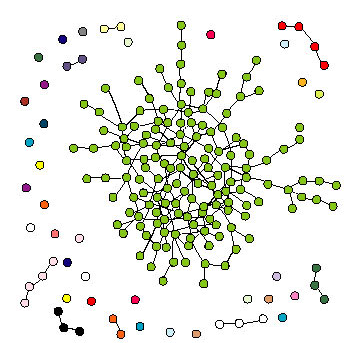
\includegraphics[scale=0.8]{./imagens/graph_random.png}
\caption{Exemplo de rede aleat�ria \cite{strogatz2001exploring}}
\label{graph_random}
\end{figure}

Desde o trabalho pioneiro, redes aleat�rias t�m sido estudadas mais profundamente sob o aspecto matem�tico\cite{bollobas2001random}. A partir deste modelo foram criadas arquiteturas idealizadas para modelos din�micos de redes de genes, ecossistemas e a propaga��o de doen�as infecciosas \cite{strogatz2001exploring}. Outros modelos foram propostos devido � limita��o deste modelo em representar caracter�sticas de redes reais.

\subsection{Modelo Watts-Strogatz}

Redes regulares e aleat�rias s�o ambas boas idealiza��es e t�m suas aplica��es no campo da pesquisa \cite{strogatz2001exploring}, por�m, a maioria das redes reais t�m um padr�o intermedi�rio entre a ordem e a desordem. O modelo proposto por Watts e Strogatz \cite{watts1998collective}, denominado \textit{small world}, � capaz de ajustar este meio-termo a partir de uma rede regular. O nome \textit{small world} (``mundo pequeno'', em ingl�s), faz refer�ncia ao trabalho de Stanley Milgram, no qual constatou-se que, sob o ponto de vista matem�tico, quaisquer duas pessoas nos Estados Unidos est�o separadas por 5 conhecidos \cite{milgram1967small}. John Guare popularizou o termo \textit{small world} como ``Seis Graus de Separa��o'' em seu livro, considerando a premissa existencial de que quaisquer duas pessoas no mundo est�o conectadas por n�o mais do que 6 conhecidos \cite{guare1992six}.

Na interpola��o entre redes regulares e aleat�rias, � considerado o processo de religa��o aleat�ria apresentado na Figura \ref{fig:graph_world}. Considerando uma rede com a estrutura em anel contendo $N$ v�rtices e $k$ arestas por v�rtice, percorre-se todas as arestas da rede, religando-as de forma aleat�ria segundo uma probabilidade $p$. Se $p = 0$ a aresta permanecer� intacta, pois n�o existe probabilidade alguma de religa��o; no extremo oposto, com $p = 1$, a aresta ser� religada de forma aleat�ria na rede. A escolha do valor de $p$ entre $0 < p < 1$ permite variar entre uma rede aleat�ria e uma rede regular.

\begin{figure}[!htb]
\centering
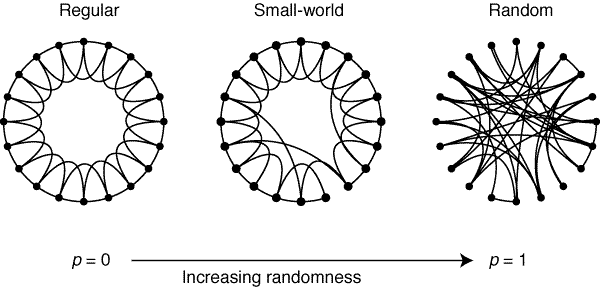
\includegraphics[scale=0.8]{./imagens/graph_world.png}
\caption{Processo de obten��o de uma rede de pequeno-mundo a partir de uma rede regular}
\label{fig:graph_world}
\end{figure}
 
As redes \textit{small world} apresentam duas propriedades importantes \cite{strogatz2001exploring}: (1) Redes altamente agrupadas - Estas redes s�o muito mais agrupadas do que redes aleat�rias. Considerando os v�rtices A, B e C, se A est� ligado a B e B est� ligado a C, ent�o existe grande probabilidade de A estar conectado a C; e (2) Caminho geod�sico m�dio baixo - A maiores dos v�rtices est�o conectados atrav�s de um caminho geod�sico de comprimento baixo. O comportamento com rela��o aos caminhos geod�sicos pode ser constatado atrav�s da Equa��o \ref{eq:caminho}, que consiste no c�lculo do caminho m�nimo m�dio entre todos os pares de v�rtices em um grafo n�o-direcionado, onde $d_{ij}$ � a dist�ncia geod�sica entre o v�rtice $i$ e o v�rtice $j$

\begin{equation}
  L = \frac{1}{\frac{1}{2} n(n+1)} \sum_{i \geq j}d_{ij}\\
  \label{eq:caminho}
\end{equation}

Matematicamente, estas propriedades podem ser evidenciadas com c�lculos estat�sticos. Primeiramente vale ressaltar que para que as propriedades sejam v�lidas assume-se que o grafo n�o possui v�rtices desconexos, necessitando que $n > k > \log (n) > 1$, no qual $k > \log (n)$ garante que um grafo aleat�rio seja conectado. 

Watts e Strogatz constataram que estas duas propriedades est�o presentes tamb�m em muitas redes naturais e tecnol�gicas \cite{watts1998collective}, como a rede neural do verme \textit{Caenorhabditis Elegans}, a rede de energia do oeste do Estados Unidos e o grafo de colabora��o entre autores em filmes. Al�m disso, constatou-se que sistemas din�micos com efeito \textit{small world} apresentam aumento na velocidade de propaga��o do sinal, poder computacional e sincroniza��o. Em geral, os caminhos m�nimos prov�m canais de comunica��o de alta velocidade entre diferentes partes do sistema, facilitando os processos din�micos, como sincroniza��o, que requer informa��o com rela��o ao estado global do sistema \cite{strogatz2001exploring}. Al�m disso, doen�as infecciosas se espalham mais rapidamente em redes de \textit{small world}.

\subsection{Modelo Barab�si-Albert}

Em redes reais, alguns n�s s�o mais conectados do que outros. No modelo proposto por Barab�si e Albert \cite{barabasi1999emergence}, denominado Livre de Escala, as redes apresentam uma ordem na din�mica de estrutura��o. As redes Livres de Escala possuem duas caracter�sticas chave presentes em redes reais: (1) Incorporam crescimento; e (2) Apresentam conex�o preferencial. A conex�o preferencial se refere � tend�ncia de um novo v�rtice conectar-se a um v�rtice de grau elevado. Estes n�s altamente conectados s�o denominados \textit{hubs}.

Barab�si e Albert afirmam que em muitos sistemas a probabilidade $P(k)$ de que um v�rtice interaja com $k$ v�rtices decai como uma Lei de Pot�ncia, sendo $P(k) \sim k^{-\gamma}$, ou seja, decai muito mais lentamente que Poisson, distribui��o de graus prevista em uma rede aleat�ria ou \textit{small world} \cite{strogatz2001exploring}. Na Lei de Pot�ncia, o expoente $\gamma$ determina a taxa de decaimento, que � tipicamente medida no intervalo $2 < \gamma < 3$. Na rede da Web, a probabilidade de $k$ documentos apontarem para uma certa p�gina segue a Lei de Pot�ncia com $\gamma = 2.1 \pm 0.1$ \cite{barabasi1995emergence}. 

Em outras palavras, uma rede aleat�ria possui grande parte dos v�rtices com n�mero de conex�es pr�ximo da m�dia da distribui��o, de forma que cada aresta est� presente ou ausente com probabilidade igual. Diferentemente, em redes livres de escala a distribui��o do grau dos v�rtices decai lentamente para a direita, formando uma "cauda", indicando que a maioria dos n�s tem grau menor que a m�dia da distribui��o \cite{watts2004new}, de forma que a probabilidade da exist�ncia de um v�rtice com grau alto � muito menor do que um v�rtice com grau baixo. Este comportamento � ilustrado na Figura \ref{comp_distr}.

\begin{figure}[!htb]
\centering
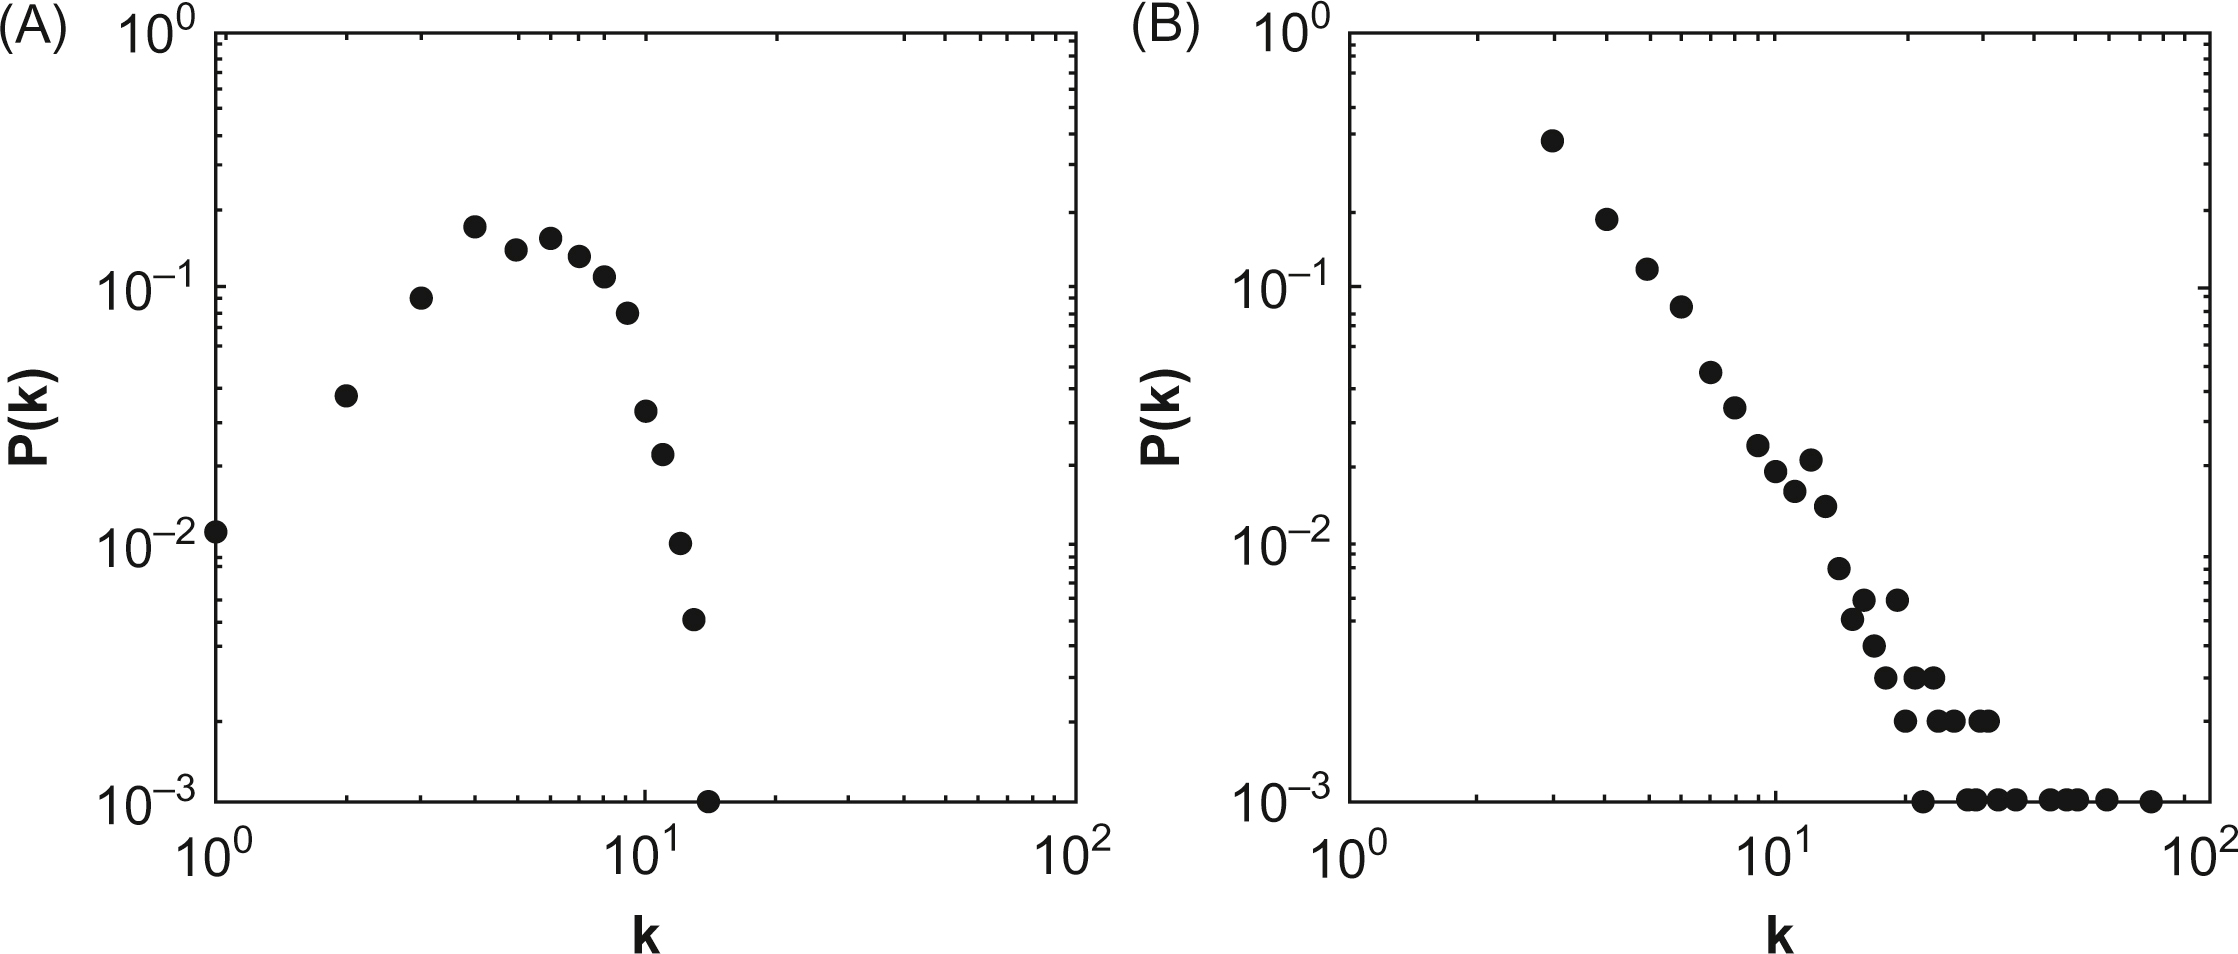
\includegraphics[scale=0.15]{./imagens/comparisson.png}
\caption{Compara��o entre a distribui��o de uma rede aleat�ria e uma rede livre de escala \cite{scott2011network}}
\label{comp_distr}
\end{figure}

Este comportamento � notado em grande parte das redes reais. No Twitter, pessoas normalmente seguem amigos e pessoas famosas que disp�em informa��es de sua vida pessoal. Em uma rede de cita��es de artigos, � evidente que pesquisadores t�m prefer�ncia em citar trabalhos conhecidos e bem publicados. Um exemplo de uma rede Livre de Escala � apresentado na Figura \ref{graph_scale}.

\begin{figure}[!htb]
\centering
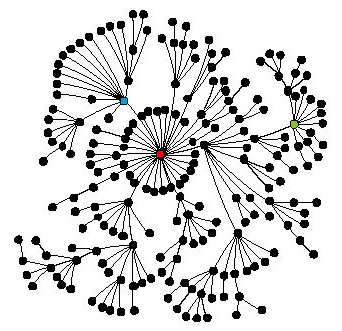
\includegraphics[scale=0.8]{./imagens/scale_free.png}
\caption{Exemplo de rede Livre de Escala \cite{strogatz2001exploring}}
\label{graph_scale}
\end{figure}

\subsection{Modelo Ravasz-Barab�si}

Muitas redes reais que modelam fen�menos naturais e sociais possuem duas propriedades gen�ricas: (1) s�o livres de escala e (2) apresentam um alto grau de agrupamento. Resultados emp�ricos mostraram que o coeficiente de agrupamento m�dio � significamente maior para redes reais do que para redes aleat�rias de mesmo tamanho. Ao mesmo tempo muitas redes cient�ficas e biol�gicas demonstraram ter a propriedade de serem livres de escala. Modelos propostos para descrever a topologia de redes complexas, em geral, t�m dificuldade em apresentar tais caracter�sticas simultaneamente.

Ravasz e Barab�si \cite{ravasz2003hierarchical} mostraram que estas duas propriedades ocorrem devido a presen�a de uma organiza��o hier�rquica. Portanto, o modelo proposto por ambos consiste em uma rede que combina a propriedade de redes Livre de Escala e de alto grau de agrupamento.

\begin{figure}[!htb]
\centering
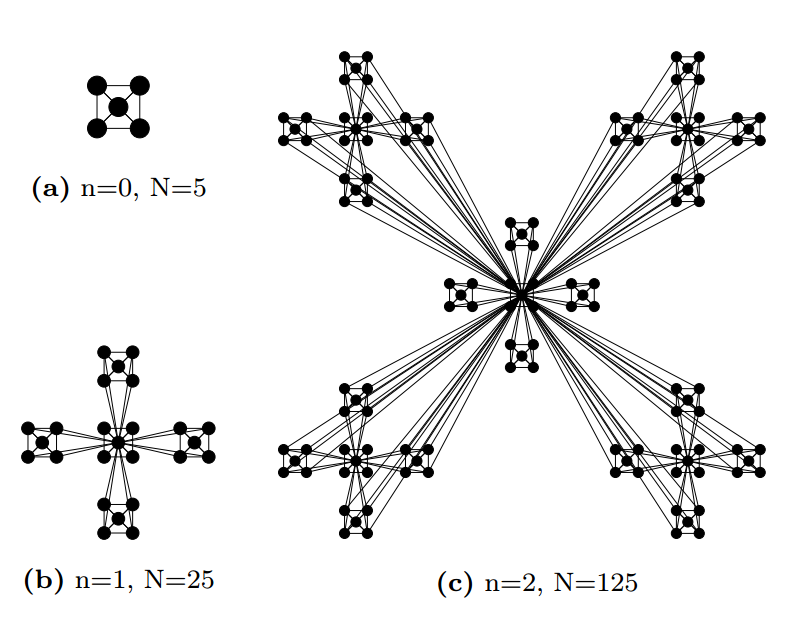
\includegraphics[scale=0.4]{./imagens/graph_h.png}
\caption{Exemplo do processo de forma��o de uma rede hier�rquica \cite{ravasz2003hierarchical}} 
\label{graph_h}
\end{figure}

\chapter{Desenvolvimento do Trabalho}

O trabalho desenvolvido consistiu em

ferramenta
experimentos
- valida��o
- modelos de rede
- datasets
- dados reais

\section{Atividades Realizadas}

\subsection{Biblioteca CGraph}

 A biblioteca CGraph \cite{cesar2013cgraph} utilizada foi implementada por um dos autores (Cesar) 
durante seu trabalho de Inicia��o Cient�fica e Mestrado, utilizando a linguagem de programa��o C89 ANSI 
em ambiente POSIX. A biblioteca foi extendida por ambos os autores para an�lise de processos de dissemina��o.

A estrutura de dados para representa��o de grafos � por meio de lista de adjac�ncias, armazenando 
toda a informa��o necess�ria em mem�ria f�sica. Para um sistema com 4 GB de mem�ria RAM e arquitetura de 
64 bits, um grafo direcionado est� limitado a menos de 500 milh�es de arestas, e um grafo n�o-direcionado 
est� limitado a menos de 250 milh�es de arestas.

A biblioteca est� em desenvolvimento, e j� possui diversos algoritmos para entrada, gera��o, m�trica e 
simula��o de grafos n�o-direcionados, apresentados a seguir:

\begin{itemize}
 \setlength{\itemsep}{0.0\baselineskip}
 \item Leitura de \textit{datasets}.
 \item Inser��o de arestas, extra��o de subgrafo.
 \item Extra��o de componentes.
 \item M�tricas de centralidade: grau, intermedia��o, proximidade, autovetor, PageRank e $k$-core.
 \item C�lculo de dist�ncia geod�sica.
 \item Assortatividade.
 \item Modelos de rede: grafo completo, Erd�s-R�nyi, Barab�si-Albert, Watts-Strogatz, Ravasz-Barab�si.
 \item Layout com sa�da SVG: aleat�rio, circular, circular ordenado por grau, definido pelo usu�rio.
 \item Modelos de dissemina��o: SI, SIS, SIR, SEIR, Daley-Kendall, Zumbi.
\end{itemize}

Os modelos de dissemina��o comportam apenas o caso de \emph{dissemina��o s�ncrona}, onde a cada
passo de tempo todos os individuos computam seu pr�ximo estado, levando em conta seu estado atual e
uma poss�vel intera��o com um indiv�duo infeccioso. Ainda n�o s�o suportados (1) mais que
um estado infeccioso, (2) infec��o m�ltipla a partir de um �nico infeccioso \cite{borge2012locating} ou 
(3) modelos ass�ncronos, onde apenas um indiv�duo infeccioso transmite por turno.

A simula��o � realizada de forma abstra�da: a fun��o \texttt{graph\_propagation\_t}
executa os passos, contando o n�mero de indiv�duos infecciosos e escolhendo uniformemente entre seus
adjacentes com quem ele interage. O modelo de propaga��o, representado na estrutura 
\texttt{graph\_propagation\_model\_t}, deve implementar dois \textit{callbacks} para a 
execu��o da propaga��o, de forma semelhante � especializa��o em orienta��o a objeto:

\begin{itemize}
 \item \texttt{graph\_transition\_t}: Determina a transi��o dos indiv�duos, dependendo do estado atual e 
       das intera��es escolhidas.
 \item \texttt{graph\_is\_end\_t}: Determina se a propaga��o j� atingiu um estado estacion�rio.
\end{itemize}

\subsection{Valida��o da simula��o}

Modelos de dissemina��o podem ser compreendidos como um processo discreto ou 
cont�nuo. Em um processo discreto, cada indiv�duo encontra-se em um dado estado, transitando em instantes
discretos conforme o estado dos seus vizinhos e de acordo com certas probabilidades. No processo cont�nuo, tais 
probabilidades s�o vistas como taxas de transi��o entre compartimentos, e o comportamento do processo �
obtido solucionando-se equa��es diferenciais. 

Espera-se que o resultado obtido em uma solu��o do modelo diferencial corresponda �quele observado em um 
grafo completo com um n�mero infinito de v�rtices; na pr�tica, bastam algumas centenas de v�rtices para
se obter comportamentos semelhantes. 

O modelo discreto � solucionado sobre um grafo completo com $N=500$ v�rtices, com crit�rio de parada de que 
nenhum v�rtice esteja no estado infeccioso. Tal crit�rio n�o pode ser satisfeito para o modelo SIS sem um 
tempo de processamento muito longo, ent�o a simula��o � interrompida arbitrariamente ap�s 90 itera��es\footnotemark.

\footnotetext{Este limite corresponde a um limite codificado na biblioteca de propaga��o, onde o n�mero de
itera��es � limitado a $10 \log_2 N$, para evitar simula��es onde a condi��o de parada � muito improv�vel ou
mesmo imposs�vel.}

Para solucionar o modelo cont�nuo, empregamos um m�todo de Runge-Kutta de ordem 2 com passo de tempo
$h=10^{-3}$. Definimos a propor��o inicial de suscet�veis em $s_0 = 1-1/N$, e a de infectados em $i_0 = 1/N$. 
Definimos o crit�rio de parada como satisfazer a inequa��o $|i - i_\infty| < 1/N$, onde $i$ � a propor��o de 
indiv�duos no estado infeccioso e $i_\infty$ � a solu��o anal�tica para $t \to \infty$. 

Utilizamos os par�metros $\alpha=1$, $\beta=1/2$ e $\gamma=1$ para a solu��o num�rica e para a
simula��o em grafo, quando apropriado. Executamos 50 repeti��es da simula��o, e calculamos a m�dia e 
desvio padr�o do n�mero de passos e da propor��o final de suscet�veis. Os resultados est�o mostrados na 
Tabela \ref{tab:valida-simulacao}. Os dois modelos s�o em geral equivalentes, exceto por incompatibilidades
no tempo de propaga��o do modelo SIS e na propor��o de suscet�veis do modelo Daley-Kendall. As causas 
destas discrep�ncias n�o foram examinadas. 

\begin{table}[!htb]
 \centering
 \caption{Compara��o entre solu��o diferencial e simula��o em grafo completo}\label{tab:valida-simulacao}
 \begin{tabular}{|l|c|cc|cc|}
  \hline
  \multirow{2}{*}{Modelo} & \multirow{2}{*}{$s_\infty$ (\%)} & \multicolumn{2}{c|}{Diferencial} & \multicolumn{2}{c|}{Simula��o} \\ \cline{3-6}
                          &                                    & Tempo & Suscet�veis (\%)         & Tempo        & Suscet�veis (\%) \\ \hline
  SI                      &  0.0000                            & 12.4  & 0.20                     & 17.2$\pm$1.3 & 0.00             \\
  SIS                     &  50.000                            & 22.1  & 50.2                     &              & 49.9$\pm$2.3     \\
  SIR                     &  20.389                            & 32.5  & 20.4                     & 32.3$\pm$3.4 & 20.5$\pm$2.7     \\
  SEIR                    &  20.389                            & 44.2  & 20.4                     & 47.0$\pm$5.6 & 20.2$\pm$2.9     \\
  Daley-Kendall           &  5.8924                            & 22.5  & 5.98                     & 24.6$\pm$2.8 & 8.4$\pm$1.5      \\ \hline
 \end{tabular}
\end{table}

\subsection{Propaga��o em \textit{datasets}}

O estudo de dissemina��o em redes reais permite visualizar o impacto das diversas propriedades estruturais no sucesso de uma propaga��o.
Se por um lado redes reais possuem diversas caracter�sticas dif�ceis de serem replicadas em modelos, por outro � dif�cil comparar 
o comportamento entre as mesmas.

As redes utilizadas para uma simula��o de propaga��o s�o descritas a seguir. Todas foram tratadas como n�o-direcionadas.

\begin{itemize}
 \item \texttt{macaque}: Rede cortical de um macaco;
 \item \texttt{cat}: Rede cortical e tal�mica de um gato;
 \item \texttt{mangdry}, \texttt{mangwet}: Rede alimentar do Estu�rio Mangrove nas temporadas de seca e chuva;
 \item \texttt{baydry}, \texttt{baywet}: Rede alimentar da ba�a da Fl�rida nas temporadas de seca e chuva;
 \item \texttt{email}: Rede de contatos de e-mail de membros da Universitat Rovira i Virgili (Tarragona);
 \item \texttt{powergrid}: Rede de transmiss�o el�trica no leste dos Estados Unidos;
 \item \texttt{pgp}: Rede de confian�a do esquema de criptografia PGP;
 \item \texttt{astrophysics}: Rede de colabora��o na �rea de Astrof�sica;
 \item \texttt{internet}: Rede de roteadores da Internet no n�vel de Sistemas Aut�nomos;
 \item \texttt{enron}: Rede de contatos de e-mail da companhia Enron;
 \item \texttt{15m}: Rede de contatos dos participantes do movimento espanhol 15 de Mayo no Twitter.
\end{itemize}

 As m�tricas realizadas sobre cada rede, que esperamos que tenham impacto sobre o sucesso de uma propaga��o s�o
\begin{itemize}
 \item N�mero de v�rtices $N$. 
 \item Grau m�dio $\langle k \rangle$. 
 \item Coeficiente de agrupamento m�dio $\langle C \rangle$. 
 \item Assortatividade $r$.
 \item M�ximo \textit{$k$-core} $\kappa$.
\end{itemize}

 Realizamos 50 repeti��es do modelo de propaga��o SIR com par�metros $\alpha = 1$ e $\beta = 1/2$ para cada \textit{dataset}, 
e calculamos a m�dia e desvio padr�o do tempo de propaga��o e da propor��o final de suscet�veis. As m�tricas e resultados 
destas simula��es est�o registradas na Tabela \ref{tab:dataset-simulation}.

\begin{table}[!htb]
 \centering
 \caption{Execu��o em datasets}\label{tab:dataset-simulation}
 \begin{tabular}{|l|ccccc|cc|}
  \hline
     \textit{dataset} & $N$   & $\langle k \rangle$ & $\langle C \rangle$ & $r$    & $\kappa$ & Tempo            & Suscet�veis (\%) \\ \hline
     \texttt{macaque} & 94    & 32.2                & 0.774               & -0.391 & 28       & $21.30 \pm 6.5$  & $38.72 \pm 16.6$ \\
         \texttt{cat} & 95    & 24.6                & 0.615               & -0.140 & 19       & $21.46 \pm 7.0$  & $41.77 \pm 18.6$ \\
     \texttt{mangdry} & 97    & 29.8                & 0.461               & -0.532 & 23       & $21.98 \pm 4.2$  & $33.03 \pm 11.5$ \\
     \texttt{mangwet} & 97    & 29.8                & 0.468               & -0.539 & 23       & $21.74 \pm 5.1$  & $35.81 \pm 14.3$ \\
      \texttt{baydry} & 128   & 32.9                & 0.335               & -0.133 & 24       & $23.76 \pm 6.8$  & $37.08 \pm 17.1$ \\
      \texttt{baywet} & 128   & 32.4                & 0.335               & -0.157 & 23       & $23.98 \pm 5.5$  & $32.20 \pm 11.6$ \\
       \texttt{email} & 1133  & 9.62                & 0.221               & +0.112 & 11       & $41.90 \pm 14.5$ & $64.16 \pm 12.3$ \\
   \texttt{powergrid} & 4941  & 2.67                & 0.080               & -0.073 & 5        & $12.54 \pm 8.5$  & $99.71 \pm 0.3$  \\
         \texttt{pgp} & 10680 & 4.55                & 0.266               & +0.178 & 31       & $9.82  \pm 11.6$ & $99.83 \pm 0.8$  \\
    \texttt{internet} & 22963 & 4.22                & 0.230               & -0.041 & 25       & $37.26 \pm 20.1$ & $99.13 \pm 0.6$  \\
\texttt{astrophysics} & 16706 & 16.1                & 0.670               & +0.452 & 56       & $62.22 \pm 26.5$ & $75.99 \pm 10.6$ \\
       \texttt{enron} & 36692 & 10.7                & 0.509               & -0.101 & 43       & $41.00 \pm 33.0$ & $95.32 \pm 4.4$  \\
         \texttt{15m} & 87569 & 109.9               & 0.224               & -0.164 & 185      & $72.26 \pm 5.4$  & $80.19 \pm 0.3$  \\ \hline
 \end{tabular}
\end{table}

Redes assortativas tendem a ser mais resilientes a ataques direcionados, de modo que se alguns 
\textit{hubs} tornarem-se refrat�rios � dissemina��o (por exemplo, no estado Removido do modelo
SIR), a dissemina��o persiste se outros \textit{hubs} se mantiverem infecciosos. Do contr�rio,
redes desassortativas tendem a se tornarem desconectadas quando alguns \textit{hubs} s�o 
removidos, de modo que a infec��o pode falhar em atingir todos os indiv�duos.

Alguns \textit{datasets} (\texttt{powergrid}, \texttt{pgp}, \texttt{internet}) apresentam propaga��o extremamente ineficiente, com praticamente 
todos os indiv�duos permanecendo suscet�veis. As causas deste comportamento n�o est�o claras, uma vez que as m�tricas estudadas n�o apontam para
uma classifica��o comum para estas redes. Mais experimentos devem ser realizados, variando a propor��o de n�s infectados iniciais e suas posi��es
relativas na rede.

\subsection{Compara��o de propaga��o entre modelos de rede equivalentes}

Nesta etapa do trabalho foram feitos experimentos para evidenciar as caracter�sticas instr�nsicas dos modelos de rede. Foi fixado um modelo de propaga��o, para que os resultados obtidos atrav�s da propaga��o de informa��o em diferentes modelos pudessem ser comparados. Os resultados calculados s�o: (1) tempo de propaga��o de uma informa��o na rede e (2) o alcance da propaga��o. O alcance da propaga��o consiste no n�mero de v�rtices que receberam a informa��o.

Para a execu��o dos experimentos foi escolhido o modelo SI (Suscet�vel-infectado), dado que � um modelo mais determin�stico. Em outros modelos como o SIR e o SIS, a propaga��o pode extinguir-se de forma inesperada, pois os n�s infectados podem retornar ao estado suscet�vel ou recuperado. Com exce��o do modelo Ravasz-Barab�si, o n�mero de v�rtices $N$ foi fixado em 10 mil e o grau m�dio $\langle k \rangle$ foi fixado em 9. A escolha do grau m�dio se deu pela condi��o para que um grafo aleat�rio n�o possua componentes desconexos, sendo $k > \log(N)$. A propaga��o da informa��o nos modelos � repetida 1000 vezes, para que seja analisado o comportamento m�dio da propaga��o para cada modelo de rede. Os resultados da execu��o dos experimentos s�o apresentados na Tabela \ref{tab:network-model}.

\begin{table}[h]
 \label{tab:network-model}
 \caption{M�tricas das redes para os modelos apresentados}
 \centering
  \begin{tabular}{lcccc}
   \hline
	&	ER	&	WS	&	BA	&	RB	\\ \hline
Tempo de propaga��o(ms)	&	136,3	&	36,7	&	81,3	&	65,2	\\
M�dia de infectados	&	9999,0	&	10000,0	&	10000,0	&	6726,2	\\
Desvio Padr�o de infectados	&	0,1	&	0,0	&	0,0	&	203,0	\\
M�dia de suscetivos	&	1,0	&	0,0	&	0,0	&	1049,8	\\
Desvio Padr�o de suscetivos	&	0,1	&	0,0	&	0,0	&	203,0	\\
M�dia de mensagens	&	1053834,9	&	251095,4	&	451380,0	&	465174,9	\\
Desvio Padr�o de mensagens	&	19588,1	&	35222,9	&	82172,8	&	28969,0	\\
M�dia de itera��es	&	134,0	&	55,3	&	73,1	&	131,0	\\
Desvio Padr�o de itera��es	&	0,0	&	4,0	&	8,5	&	0,0	\\
Agrupamento m�dio	&	0	&	0,133	&	0,008	&	0,825	\\
Caminho m�nimo m�dio	&	5,33	&	5,938	&	3,474	&	3,776	\\
Di�metro	&	10	&	9	&	5	&	10	\\ \hline

  \end{tabular}
 \end{table}

Atrav�s da an�lise do tempo de propaga��o, percebe-se o modelo de WS teve uma propaga��o muito mais r�pida que os demais modelos. Isto se deve as propridades de \textit{small world}. Este modelo propagou a informa��o para toda a rede com o menor n�mero de passos e o menor n�mero de mensagens. O segundo modelo que propagou a informa��o mais rapidamente foi o BA, o qual possui a propriedade de redes livres de escala. Um fato importante em redes livres de escala � que estas tamb�m t�m a propriedade \textit{small world} \cite{watts1999small}. A proprieade \textit{small world} � notada em livres de escala dado que o di�metro de uma rede $d$ cresce em escala logar�tmica em rela��o ao n�mero de n�s $N$ \cite{kosmidis2007propagation}.

Ao contr�rio dos dois primeiros modelos analisados, os modelos ER e RB tiveram o n�mero de passos limitado pelo crit�rio de parada. O crit�rio de parada consiste em $K \log_2(N)$. A l�gica � que uma propaga��o "perfeita" necessita de $\log_2(N)$ passos. Atrav�s desta fun��o a progress�o de infectados teria ordem quadr�tica, totalizando $\log_2(N)$ passos. O $k$ consiste em um par�metro de seguran�a. Portanto, nota-se que RB possui um tempo de propaga��o menor que BA, por�m, cerca de 14\% da rede n�o recebeu a informa��o. Analisando-se o di�metro da rede, fica claro que as modelos ER e RB, que atingiram o limite de passos, possuem um di�metro de rede maior.

Em geral, a principal propriedade da rede WS consiste no comportamente m�dio entre redes aleat�rias e regulares. Isto permite que a rede seja altamente agrupada (como em redes regulares) e manter a caracter�stica de caminhos m�nimos. Estas caracter�sticas, combinadas a um di�metro menor, mostram que as caracter�sticas de uma rede \textit{small eorld} s�o muito favor�veis a propaga��o de informa��o. Vale notar tamb�m que, sem o limite de execu��o pelo n�mero de passos, o modelo RB tem um comportament pr�ximo de BA. 

Analisando-se RB, Ravasz e Barab�si \cite{ravasz2003hierarchical} afirmam que as principais caracter�sticas deste modelo consiste no alto grau de agrupamento e comportamento livre de escala. Wang et al \cite{fu2007information} realizaram diversos experimentos de propaga��o de informa��o com o modelo SIR em redes hier�rquicas. Os resultados demonstraram que o alcance da propaga��o depende da localiza��o do indiv�duo que inicia a mesma. Wang et al constataram que o alcance � m�ximo ocorre quando o v�rtice escolhido inicialmente est� em uma camada intermedi�ria. Os resultados das simula��es indicaram que a melhor estrat�gia para propagar uma informa��o consiste em fazer com que indiv�duos em camadas intermedi�rias recebam a informa��o e espalhem esta ao seus vizinhos. Portanto, o comportamento verificado nos experimentos realizados neste n�o � anormal.

\subsection{Gripe de Hong Kong}

A Gripe de Hong Kong foi a terceira pandemia de gripe do s�culo XX. Esta gripe foi uma pandemia de categoria 2, segundo o �ndice de Severidade de Pandemia (PSI), que consiste em uma classifica��o para reportar a severidade de uma pandemia nos Estados Unidos, de forma que a categoria 1 � mais branda, enquanto a categoria 5 indica o pior caso de severidade. Os surto ocorreu  entre 1968 e 1969 e matou aproximadamente 1 milh�o de pessoas pelo mundo \cite{paul2008fundamental}.

A causa desta pandemia foi o aparecimento de uma nova varia��o do v�rus Influenza A (H3N2), que deu origem a um novo subtipo. Esta variante antig�nica produziu em Hong Kong, em meados de Julho, uma epidemia de grande extens�o, que se espalhou pelo mundo. Em setembro a pandemia j� havia alcan�ado �ndia, Filipinas, Austr�lia e Europa. Neste mesmo m�s as tropas norte-americanas em miss�o na Guerra do Vietnam, contra�ram o v�rus e o levaram para os Estados Unidos.

Nos EUA, os primeiros casos foram detectados na Calif�rnia, de onde a epidemia se propagou rapidamente, estando em Dezembro em todos os Estados. Em todos os pa�ses, com exce��o dos EUA, a doen�a foi benigna, n�o estando associada a grande n�mero de mortes. Um relat�rio divulgado pela Congressional Quarterly, em 1986, afirmou que quase 50 milh�es de pessoas foram infectadas nos Estados Unidos e aproximadamente 33.800 morreram \footnote{Dispon�vel em:  http://www.flu.gov/pandemic/history/}.

Durante o per�odo de infec��o a popula��o podia ser dividida em 3 categoria:

\begin{itemize}
\setlength{\itemsep}{0.0\baselineskip}
\item Pessoas infectadas pela gripe;
\item Pessoas que se recuperaram;
\item Pessoas que n�o foram infectadas.
\end{itemize}

Sabendo-se da aplica��o de dissemina��o de informa��o no contexto de propaga��o de epidemias, modelou-se o problema segundo o modelo epidemiol�gico SIR (Suscet�vel - infectado - recuperado). Os valores utilizados nos experimentos foram obtidos atrav�s da observa��o da evolu��o da doen�a na cidade de Nova Iorque, que na �poca contava com uma popula��o de aproximadamente 7,9 milh�es de pessoas. Os dados s�o os seguintes:

\begin{itemize}
\setlength{\itemsep}{0.0\baselineskip}
\item Inicialmente t�m-se 7,9 milh�es de pessoas, sendo 10 infectados rferente as tropas norte-americanas voltando da guerra. 
  \begin{itemize}
  \item $S + I + R = N = 7.9$ milh�es
  \end{itemize}
\item Adimensionalizado-se o sistema, tem-se $s + i + r = 1$
  \begin{itemize}
  \item $S(0) \cong 1$
  \item $I(0) = 10/7.900.000 \cong 1.27*10^{-6}$
  \item $R(0) = 0$
  \end{itemize}
\item Per�odo de infec��o ($p_i$): 3 dias
  \begin{itemize}
  \item Taxa de recupera��o ($\beta$): $1/p_i = 1/3$
  \end{itemize}
\item Em m�dia, uma nova pessoa � infectada cada dia
  \begin{itemize}
  \item Taxa de infec��o ($\alpha$): $1/2$
  \end{itemize}
\end{itemize}

Os experimentos realizados para as simula��es da propaga��o desta pandemia em uma rede, foi feita com uma pequena parte da rede social do Facebook \cite{}. Esta rede foi escolhida devido a sua conformidade com uma rede de contato, dado que os v�rtices s�o pessoas e as arestas consistem em um relacionamente de "amizade" entre esats pessoas. Segundo Ravasz e Barab�si \cite{ravasz2003hierarchical}, redes reais apresentam a coexist�ncia de caracter�sticas intr�nsecas de modelos de rede, como o alto grau de agrupamento e a exist�ncia de caminhos geod�sicos. A rede do Facebook utilizada � n�o-direcionada e possui 1912 v�rtices e 26749 arestas. Dimensionalizando-se o problema para esta simula��o, $S(o)$ foi 1, dado que $s$ � muito pequeno e 1 � o valor m�nimo necess�rio para se iniciar uma dissemina��o de doen�a infecciosa. A Tabela \ref{tab:facebook}

 \begin{table}[h]
 \label{tab:facebook}
 \caption{Informa��es sobre a propaga��o da Gripe de Hing Kong na rede do Facebook}
 \centering
  \begin{tabular}{lcccc}
   \hline
   	&	&N�mero de itera��es	\\ \hline
	&	100	&	1000	&	10000	\\ \hline
M�dia de infectados	&	9,3	&	9,0	&	9,0	\\
Desvio Padr�o de infectados	&	1,2	&	0,0	&	0,0	\\
M�dia de suscetivos	&	1817,4	&	1842,0	&	1842,0	\\
Desvio Padr�o de suscetivos	&	135,1	&	125,6	&	125,6	\\
M�dia de recuperados	&	85,3	&	61,0	&	61,0	\\
Desvio Padr�o de recuperados	&	134,6	&	125,6	&	125,6	\\
M�dia do total de infec��es	&	254,1	&	183,7	&	183,7	\\
Desvio padr�o do total de infec��es	&	408,2	&	383,7	&	383,7	\\ \hline
  \end{tabular}
 \end{table}

Atrav�s da simula��o com os par�metros acerca da infec��o, percebe-se que a epidemia nos Estados Unidos, de fato, n�o foi t�o severa como outras pandemias como a gripe Espanhola. Percebe-se que a epidemia se estabiliza com um n�mero baixo de infectados, ou seja, dadas as tentativas de infec��o, grande maioria se recupera, ou h� infec��o em pessoas j� contaminadas. A grande aplica��o de dissemina��o de epidemias para a �rea da sa�de consiste no c�lculo de vacina��o em massa para controle de epidemias


\subsection{Sobreviv�ncia ao Apocalipse Zumbi}

\section{Resultados Obtidos}

\chapter{Conclus�o}

\section{Contribui��es}



\section{Trabalhos Futuros}




% % Usado se voc� quiser utilizar mais de uma refer�ncia que n�o foi citado no texto
% \nocite{*}

\bibliographystyle{abnt-alf}
\bibliography{referencias}

\apendice
\chapter{}



\end{document}